\section{Overview: High‐level components and their interaction}

TrackMe is a System that stores User data and makes them available for Third Parties through the requests mechanism. It also offers the in-house services Track4Run and AutomatedSOS to the end Users. In order to provide these services, the System needs two different client applications: 

\begin{itemize}[leftmargin=*]
        \item{a Mobile client that sends new User data to the server, designed specifically for individual users;}
        \item{a Web client, accessible to verified Third Parties only, that gives access to the specifically requested data.}
\end{itemize}

\begin{figure}[H]
	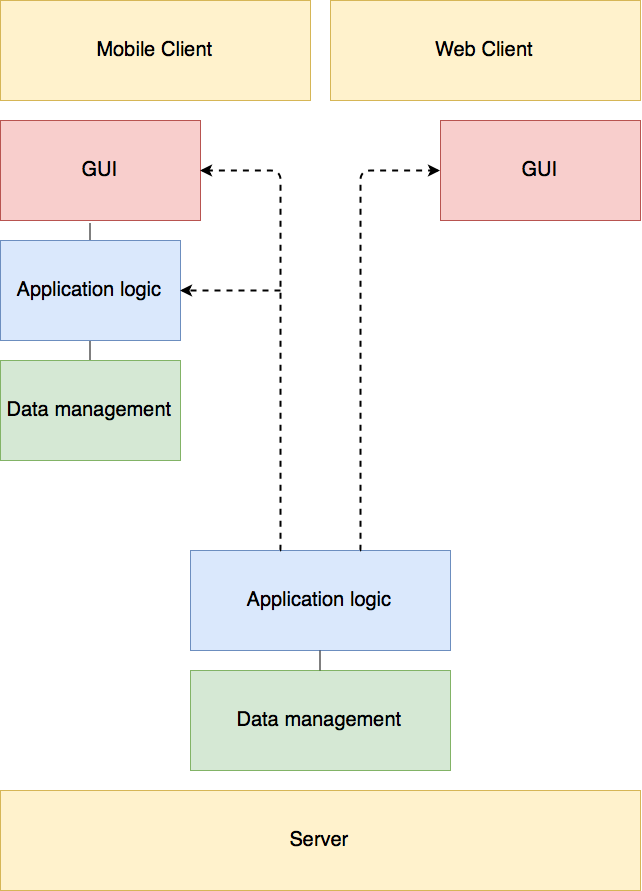
\includegraphics[scale=0.3,keepaspectratio]{./Pictures/arch-design.png}
	\centering
	\caption{Overview of the \textit{TrackMe} system}
\end{figure}

\newpage

The picture above describes the client-server architecture of the System. The Mobile and Web clients are different in terms of thickness: ithe Mobile client is provided with data management capabilities in order to 
\begin{itemize}
	\item[--] manage the collected data that have not been uploaded yet (high offline reliability)
	\item[--] store a bigger set of data and send it to the server once, instead of having multiple forwardings (low battery consumption) 
\end{itemize}
, while the Web client only shows the data that is available to be accessed by the Third Party. 

%\vskip\bigskipamount

\vspace{5mm}

\begin{figure}[H]

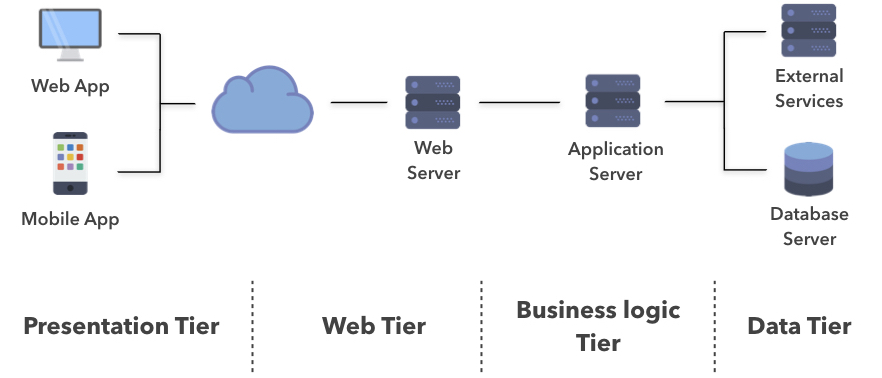
\includegraphics[scale=0.43,keepaspectratio]{./Pictures/high-level-basic.jpeg}
\centering
\caption{High-level architecture of the \textit{TrackMe} system}

\end{figure}

\vspace{5mm}

The high-level architecture of the TrackMe system is divided into four tiers:
\begin{enumerate}
\item the \textit{Presentation tier} enables the interaction with end Users, includes a Web application for Third Party access and a Mobile application, utilized by individual Users.
\item the \textit{Web tier} consists of an Apache web server that manages RESTful HTTPS requests between clients and the application server.
\item the \textit{Business Logic tier} includes the application server, where the main tasks, such as the request management, the run creation and the emergency call, will be effectively executed. 
\item the \textit{Data tier} manages the storage of the data needed for the functioning of the TrackMe system. It includes also the external services that will be required for the System to function properly.
\end{enumerate}

\newpage